\documentclass[11pt]{article}
\usepackage{amssymb}
\usepackage{amsthm}
\usepackage{amsmath}
\usepackage{listings}
\usepackage{color}
\usepackage{graphicx}
\usepackage[margin=1.0in]{geometry}

\lstdefinestyle{matlab-style}{
language=Matlab,
basicstyle=\scriptsize\ttfamily,
tabsize=2,
rulecolor=,
language=matlab,
basicstyle=\scriptsize,
aboveskip={1.5\baselineskip},
columns=fullflexible,
showstringspaces=false,
extendedchars=true,
breaklines=true,
prebreak = \raisebox{0ex}[0ex][0ex]{\ensuremath{\hookleftarrow}},
frame=single,
showtabs=false,
showspaces=false,
showstringspaces=false,
identifierstyle=\ttfamily,
keywordstyle=\color[rgb]{0,0,1},
commentstyle=\color[rgb]{0.133,0.545,0.133},
stringstyle=\color[rgb]{0.627,0.126,0.941},
keepspaces=true,
numbers=left,
numbersep=5pt,
numberstyle=\tiny\color[rgb]{0.5,0.5,0.5},
stepnumber=1
}

\newcommand{\bs}[1] {\boldsymbol{#1}}

\title{Design of an optimal wing spar\\MANE 6963 - Project 2}
\author{ID: 2168}
\date{}

\begin{document}

\maketitle
\tableofcontents
\newpage

\section{Executive summary}

\begin{figure}[hbt]
\centering
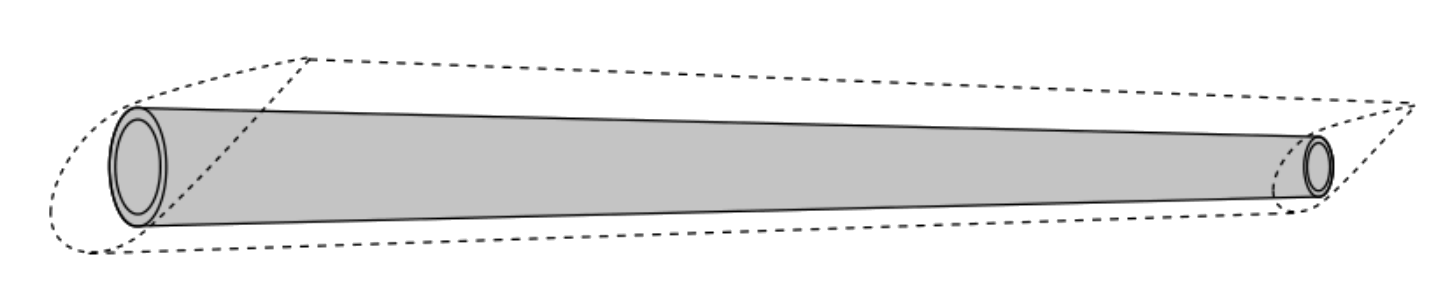
\includegraphics[width=0.6\textwidth]{spar}
\label{fig:spar}
\caption{Wing (dotted lines) and illustration of spar geometry}
\end{figure}

In this report, we investigate the optimal design of a
spar as the primary support for the wing of an aircraft.
Figure \ref{fig:spar} shows an illustration of the spar
that is to be designed. Our main objective is to minimize the
weight (and thus the mass) of the wing spar subject to
operational assumptions about the aircraft,
engineering design assumptions, and engineering
design constraints. These assumptions and
constraints are outlined below.

\subsection{Aircraft operational assumptions}

We assume that the total mass of the aircraft
is $m_{\text{plane}} = 500$ kg and that the weight
of the plane is equally supported by two wings.
Additionally, we assume that the plane is operating
at a $2.5$ g maneuver, where the span-wise force
distribution acting on the wing (and thus on the spar)
varies linearly, vanishing at the wing tip. The
distribution of this force per unit area $q(x)$
acting on the spar is shown in Figure \ref{fig:load}.

\begin{figure}[hbt]
\centering
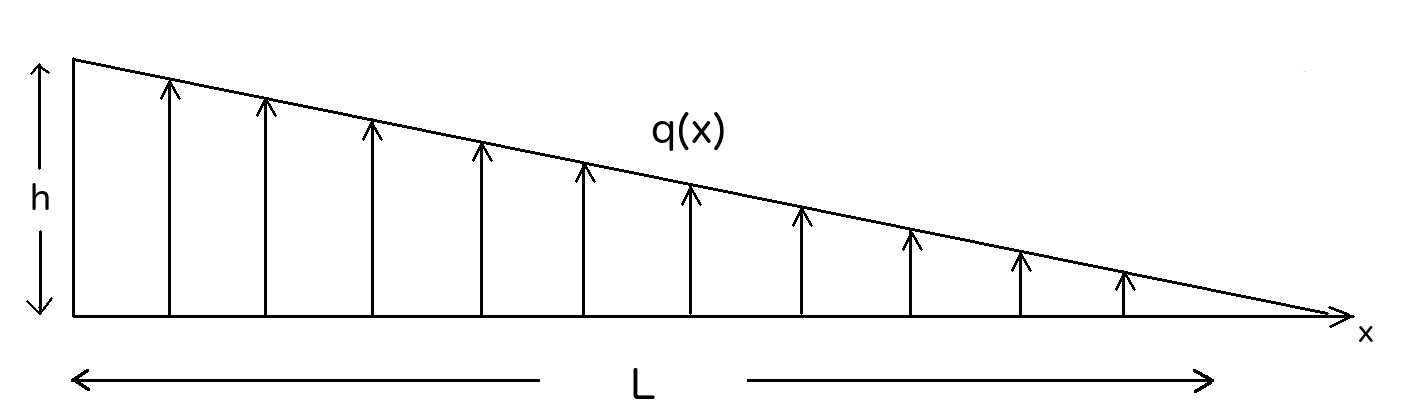
\includegraphics[width=0.6\textwidth]{load}
\caption{Load imposed on the wing}
\label{fig:load}
\end{figure}

\subsection{Engineering design assumptions}

We assume that the wing semi-span $L$ is $7.5$ m,
and that the spar supporting the wing will be made
of a composite fiber material. The material properties
of the composite are listed in Figure \ref{fig:materials}.
Additionally, we assume that the cross-section of
the spar in the $yz$ plane is a circular annulus,
as shown in Figure \ref{fig:annulus}.

\begin{figure}[hbt]
\centering
\begin{tabular}{ | l | r  |}
\hline
Material property & Value \\ \hline
Density $(\rho)$ & $1600$ km/m$^3$ \\ \hline
Young's modulus $(E)$ & $70$ GPa \\ \hline
Ultimate yield strength $(Y)$ & $600$ MPa \\ \hline
\end{tabular}
\caption{Material properties of the spar}
\label{fig:materials}
\end{figure}

\subsection{Engineering design constraints}

Due to material manufacturing constraints, we
assume that the inner radius of the spar at all
points is greater than or equal to $1$ cm, $r^i \geq 1$ cm,
and that the inner and outer radii of the spar cannot be
more than $2.5$mm apart, $r^o - r^i \geq 2.5$ mm.
Because the spar must remain within the wing, we
constrain the outer radius of the spar to be less
than or equal to $5$ cm, $r^o \leq 5$ cm.
Finally, we stipulate that the normal stress at all
span-wise locations in the be less than the yield
strength, $\sigma \leq Y$, to maintain a safe design.

\begin{figure}[hbt]
\centering
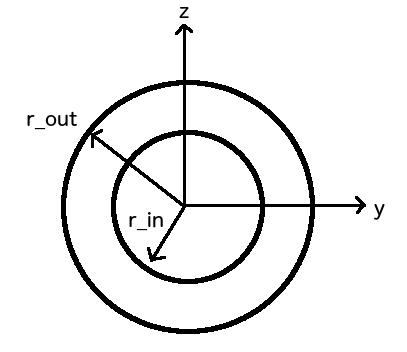
\includegraphics[width=0.3\textwidth]{annulus}
\caption{Annular cross-section of the spar geometry}
\label{fig:annulus}
\end{figure}

\subsection{Work done to achieve optimization goal}

To achieve the stated optimization goal subject to the above
constraints and assumptions, we have:
\begin{itemize}
\item Determined a suitable spar geometry parameterization,
defined by the design vector $\bs{p}$.
\item Derived the appropriate force per unit length function
$q(x)$ based on our design assumptions and implemented a Matlab
method CalcForce.m that evaluates $q(x)$ at discrete points.
\item Implemented a Matlab routine CalcMoment.m that computes
the second moment of area at cross-sections of the spar geometry.
\item Provided the functions CalcForce.m and CalcMoment.m to a
finite element analysis code to compute the normal stresses
$\sigma$ at discrete grid locations along the spar.
\item Implemented the Matlab routine CalcMass.m that computes
the mass $m$ of the spar as a function of the design variables
$\bs{p}$.
\item Implemented the Matlab routine Obj.m which computes the
mass objective function and its gradient with respect to the
design parameters $\bs{p}$ using the complex-step method.
\item Implemented the Matlab routines ConstraintLower.m,
ConstraintUpper.m, and ConstraintStress.m to effectively
impose the necessary constraints.
\item Utilized Matlab's fmincon routine, along with the methods
Obj.m, ConstraintLower.m, ConstraintUpper.m, and ConstraintStress.m,
to determine an optimal spar geometry.
\end{itemize}

In the remainder of this report, the mathematical and
implementation details of each item
in the list above are sequentially discussed.
Results of the optimization study are shown and finally
conclusions are drawn. All Matlab routines named are listed
in the Appendix.

\section{Geometry parameterization}

As stated previously, each cross-section in the $yz$ plane of the
spar geometry is assumed to be a circular annulus. We discretize
the $x$-axis using $N_x$ grid points and assume that the spar
varies piecewise linearly along the $x$-direction from grid
point to grid point. An illustration of this piecewise linearly
varying geometry is shown in Figure \ref{fig:representation}.
We parameterize this geometry by a vector $\bs{p}$
that is the concatenated values of the
inner radii values $r^i_j$ and the annular thickness
$t_j = r^0_j - r^i_j$ evaluated at discrete grid points $x_j$,
where $j=1,2,\dots,N_x$. Thus, $\bs{p} \in \mathbb{R}^{2 N_x}$
has the layout
\begin{equation}
\bs{p} = [r^i_1, r^i_2, \dots r^i_{N_x}, t_1, t_2, \dots, t_{N_x}]^T
\end{equation}

\begin{figure}[hbt]
\centering
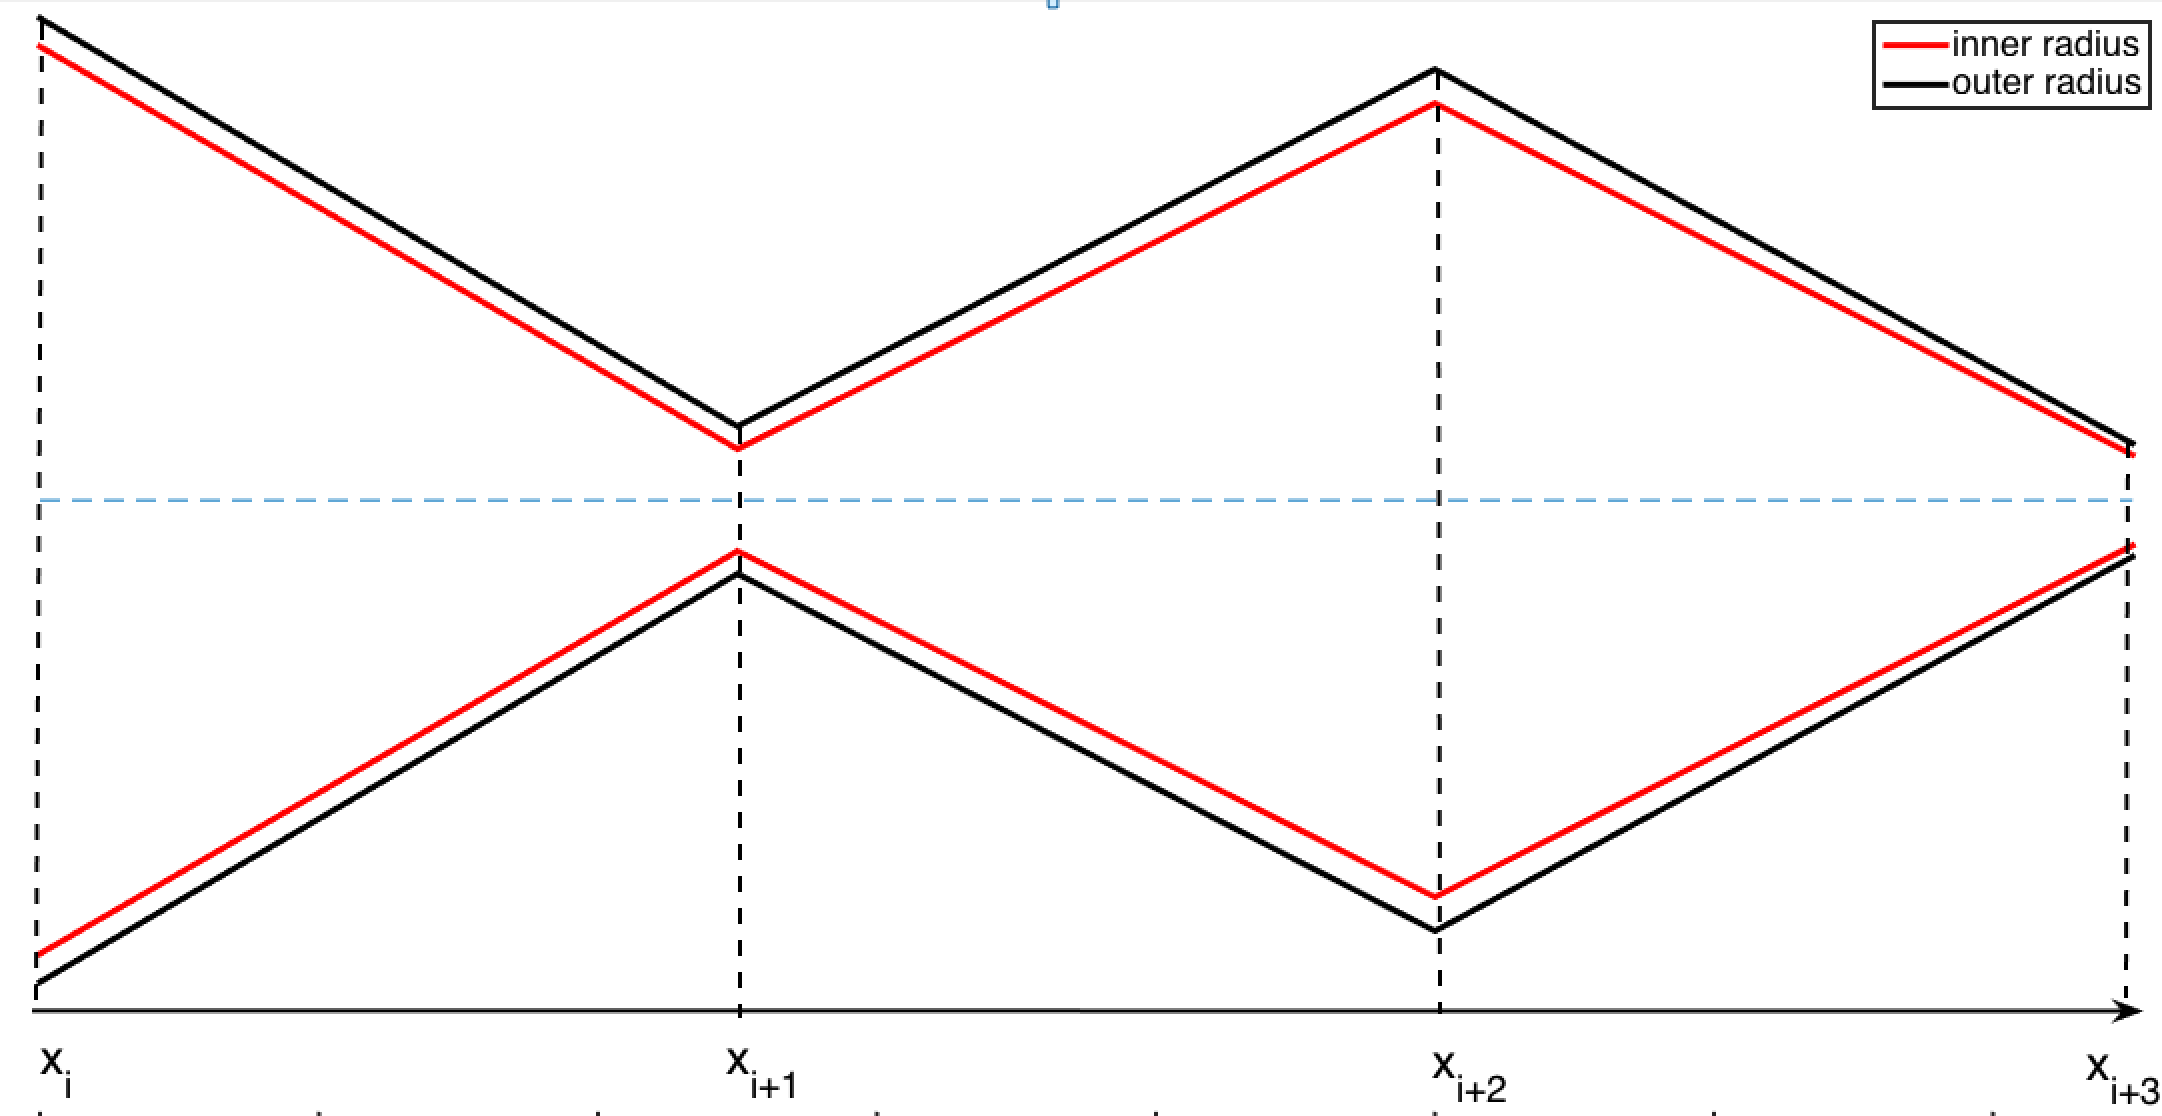
\includegraphics[width=0.5\textwidth]{representation}
\caption{Piecewise linear geometry representation}
\label{fig:representation}
\end{figure}

\section{Analysis methods}

\subsection{PDE Model}

We model the deformation of the wing spar using Euler-Bernoulli
beam theory.
\begin{equation}
\frac{d^2}{d x^2}
\left( E I_{yy} \frac{d^2 u}{dx^2} \right) =
q, \quad \forall x \in [0,L],
\end{equation}
where $I_{yy}$ is the second moment of inertia of the
cross-section of the spar and $q$ is an applied load.
We impose zero vertical or angular displacement boundary
conditions:
\begin{equation}
\begin{aligned}
u(x=0) &= 0, \\
\frac{du}{dx} (x=0) &= 0,
\end{aligned}
\end{equation}
and traction free boundary conditions at the spar tip:
\begin{equation}
\begin{aligned}
\frac{d^2 u}{dx^2} (x=L) &= 0, \\
\frac{d^3 u}{dx^3} (x=L) &= 0.
\end{aligned}
\end{equation}
Before presenting an appropriate numerical method to
solve this PDE, we first derive analytical expressions
for the load $q(x)$ and for the second moment of inertia
$I_{yy}$.

\subsection{Applied load}

It is known that the total force acting on the aircraft
during the $2.5$ g maneuver is
\begin{equation}
F = (2.5)(9.8 \text{m}\text{s}^{-2})(\frac12)(500 \text{kg}) = 6125 \text{N}.
\end{equation}
It is also known that the total force $F$ applied to the
spar is given as
\begin{equation}
F = \int_0 ^L q(x) dx,
\end{equation}
the area under the curve in Figure \ref{fig:load}, which
forms a triangular region. From geometry, we have $F = \frac12 h L$,
where $h$ is the height of the triangle. Thus, the height
of the triangular region is given as $h = \frac{2F}{L}$.
Using the well-known formula for a straight line, we conclude that
the expression for the force-per unit area is
\begin{equation}
q(x) = \frac{2F}{L} \left( 1 - \frac{x}{L} \right).
\end{equation}
The Matlab function CalcForce.m returns the value
of the force per-unit area $q(x)$ at discrete $x$
locations.

\subsection{Second moment of inertia at cross sections}

As mentioned previously, the cross-section of the spar
geometry in the $xz$ plane is a circular annulus
(see Figure \ref{fig:annulus}). The second moment
of inertia for an annulus is give by the equation:
\begin{equation}
I_{yy} = \iint z^2 \text{d} z \text{d} y.
\end{equation}
Basic calculus lead to the result:
\begin{equation}
I_{yy} = \frac{\pi}{4} \left ( (r^o)^4 - (r^i)^4 \right).
\end{equation}
The Matlab function CalcMoment.m returns the value
of $I_{yy}$ at discrete $x$-locations along the spar.

\subsection{Finite element analysis}



\section{Optimization methods}

\subsection{Computation of spar mass}

Our main objective is to minimize the weight, and thus
the mass $m$ of the spar. To compute the mass of the
spar, we first compute the spar's volume. The total volume
of the spar is computed as the sum of the volume computed
over each element in the discrete domain:
\begin{equation}
V = \sum^{N_x-1}_{j=1} V^o_j - V^i_j
\end{equation}
where $V^o_j$ denotes the volume of the truncated cone
defined by the values of the spar's outer
radii values at $x_j$ and $x_{j+1}$
\begin{equation}
{V^o}_j = \frac{\pi \Delta x}{3} ((r^o_j)^2 + (r^o_{j+1})^2 + (r^o_j)(r^i_{j+1})).
\end{equation}
Similarly, $V^i_j$ denotes the volume of the truncated cone
defined by the values of the spar's inner
radii values at $x_j$ and $x_{j+1}$.
\begin{equation}
{V^i}_j = \frac{\pi \Delta x}{3} ((r^i_j)^2 + (r^i_{j+1})^2 + (r^i_j) (r^i_{j+1}))
\end{equation}
Naturally, the difference $V^o_j-V^i_j$ denotes the
total volume associated with the element defined
by the points $x_j$ and $x_{j+1}$. The Matlab
function CalcMass.m returns the computed value
of the spar's mass, given inner and outer radii
values at discrete grid locations.

\subsection{Optimization problem statement}



\subsection{Optimization methods}

\section{Results}

\section{Conclusions}

\newpage

\section{Appendix: code listings}

\lstinputlisting[style=matlab-style,caption=CalcForce.m]{CalcForce.m}
\lstinputlisting[style=matlab-style,caption=CalcMoment.m]{CalcMoment.m}
\newpage
\lstinputlisting[style=matlab-style,caption=CalcMass.m]{CalcMass.m}
\lstinputlisting[style=matlab-style,caption=ConstraintLower.m]{ConstraintLower.m}
\newpage
\lstinputlisting[style=matlab-style,caption=ConstraintUpper.m]{ConstraintUpper.m}
\lstinputlisting[style=matlab-style,caption=ConstraintStress.m]{ConstraintStress.m}
\newpage
\lstinputlisting[style=matlab-style,caption=Obj.m]{Obj.m}
\lstinputlisting[style=matlab-style,caption=Plotter.m]{Plotter.m}
\newpage
\lstinputlisting[style=matlab-style,caption=Driver.m]{Driver.m}

\end{document}
